\subsection{Crear Tabla en la Base de Datos PostgreSQL}

Para comenzar a trabajar con PostgreSQL, primero es necesario instalar el sistema de gestión de base de datos. Para ello, se actualizan los paquetes y se instala PostgreSQL junto con sus contribuciones adicionales utilizando los siguientes comandos:

\begin{verbatim}
sudo apt update
sudo apt upgrade
sudo apt install postgresql postgresql-contrib
\end{verbatim}

Para verificar que el servicio está funcionando correctamente, se pueden utilizar los siguientes comandos:

\begin{verbatim}
sudo systemctl status postgresql
\end{verbatim}

PostgreSQL crea por defecto un usuario llamado \textit{postgres}, que actúa como superusuario del sistema de base de datos. Para comenzar a usar PostgreSQL, primero cambiamos al usuario \textit{postgres} y accedemos a la consola de PostgreSQL con:

\begin{verbatim}
sudo -i -u postgres
psql
\end{verbatim}

Una vez en la consola de PostgreSQL, procedemos a crear una nueva base de datos y una tabla dentro de esta:

\begin{verbatim}
CREATE DATABASE uoc;
\c uoc;
CREATE TABLE uoc (
    id SERIAL PRIMARY KEY,
    nombre VARCHAR(100),
    rol VARCHAR(100)
);
\end{verbatim}

Luego, poblamos la tabla con algunos datos de ejemplo:

\begin{verbatim}
INSERT INTO uoc (nombre, rol) VALUES ('Fernando', 'estudiante');
INSERT INTO uoc (nombre, rol) VALUES ('Rafael', 'profesor');
\end{verbatim}

\begin{figure}[H]
    \centering
    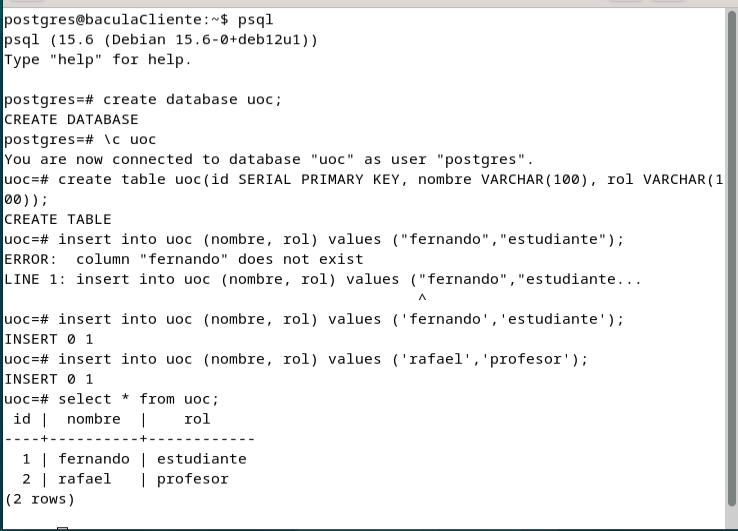
\includegraphics[width=0.5\linewidth]{instalacionBacula/postgrestCrearTabla.png}
    \caption{Creación y población de la tabla \textit{uoc} en PostgreSQL mostrando los comandos ejecutados y sus resultados.}
\end{figure}

